\documentclass[hidelinks,spanish,a4paper,14pt,oneside]{extreport}
\usepackage[utf8]{inputenc}
%\usepackage[utf8x]{inputenc}
\usepackage[spanish]{babel}
%%%%%%%%%%%%%%%%%%%%%%%%%%%%%%%%%%%%%%%%%%%%%%%%%%%%%%%%%%%%%%%%%%%%%%%%%%%%%%%
% Next 3+3 lines select PDF or PS output respectively (comment as apropriate)
% To switch from PDF and PS comment/uncomment here
% and change correspondingly the Makefile
%
\usepackage[pdftex]{color}
\usepackage[pdftex]{graphicx}
\graphicspath{{FIGURES/}}
%\usepackage[dvips]{color}
%%\usepackage[dvips]{graphicx}
%\graphicspath{{FIGURES/}}
%%%%%%%%%%%%%%%%%%%%%%%%%%%%%%%%%%%%%%%%%%%%%%%%%%%%%%%%%%%%%%%%%%%%%%%%%%%%%%%
\usepackage{alltt}
\usepackage{algorithm}
\usepackage{algorithmic}
\usepackage{multirow}
\usepackage[top=2cm, bottom=2cm, left=2cm, right=2cm]{geometry}
\usepackage{hyperref}

% Símbolo del euro
\usepackage[official]{eurosym}

%%%%%%%%%%%%%%%%%%%%%%%%%%%%%%%%%%%%%%%%%%%%%%%%%%%%%%%%%%%%%%%%%%%%%%%%%%%%%%%

% Referenciar nombres de una lista de items
\makeatletter
\let\orgdescriptionlabel\descriptionlabel
\renewcommand*{\descriptionlabel}[1]{%
  \let\orglabel\label
  \let\label\@gobble
  \phantomsection
  \edef\@currentlabel{#1}%
  %\edef\@currentlabelname{#1}%
  \let\label\orglabel
  \orgdescriptionlabel{#1}%
}
\makeatother

% Indice de referencias cruzadas
\usepackage{makeidx}
\makeindex

%%%%%%%%%%%%%%%%%%%%%%%%%%%%%%%%%%%%%%%%%%%%%%%%%%%%%%%%%%%%%%%%%%%%%%%%%%
%listings
\usepackage{listings}
\usepackage{color}
\definecolor{lightgray}{rgb}{.9,.9,.9}
\definecolor{darkgray}{rgb}{.4,.4,.4}
\definecolor{purple}{rgb}{0.65, 0.12, 0.82}
\lstdefinelanguage{JavaScript}{
  keywords={do, if, in, for, let, new, try, var, case, else, enum, eval, null, this, true, void, with, await, break, catch, class, const, false, super, throw, while, yield, delete, export, import, public, return, static, switch, typeof, default, extends, finally, package, private, continue, debugger, function, arguments, interface, protected, implements, instanceof},
  morecomment=[l]{//},
  morecomment=[s]{/*}{*/},
  morestring=[b]',
  morestring=[b]",
  ndkeywords={class, export, boolean, throw, implements, import, this},
  keywordstyle=\color{blue}\bfseries,
  ndkeywordstyle=\color{darkgray}\bfseries,
  identifierstyle=\color{black},
  commentstyle=\color{purple}\ttfamily,
  stringstyle=\color{red}\ttfamily,
  sensitive=true
}
\lstloadlanguages{Ruby}

\lstset{
   language=JavaScript,
   backgroundcolor=\color{lightgray},
   extendedchars=true,
   basicstyle=\footnotesize\ttfamily,
   showstringspaces=false,
   showspaces=false,
   numbers=left,
   numberstyle=\footnotesize,
   numbersep=9pt,
   tabsize=2,
   breaklines=true,
   showtabs=false,
   captionpos=b
}

%%%%%%%%%%%%%%%%%%%%%%%%%%%%%%%%%%%%%%%%%%%%%%%%%%%%%%%%%%%%%%%%%%%%%%%%%%%%%%%

\newcommand{\SONY}{{\sc Sony}}
\newcommand{\INTEL}{\textsf{\textsc{I}ntel}}

%%% Traducimos el pseudocodigo
\renewcommand{\algorithmicwhile}{\textbf{mientras}}
\renewcommand{\algorithmicend}{\textbf{fin}}
\renewcommand{\algorithmicdo}{\textbf{hacer}}
\renewcommand{\algorithmicif}{\textbf{si}}
\renewcommand{\algorithmicthen}{\textbf{entonces}}
\renewcommand{\algorithmicrepeat}{\textbf{repetir}}
\renewcommand{\algorithmicuntil}{\textbf{hasta que}}
\renewcommand{\algorithmicelse}{\textbf{en otro caso}}
\renewcommand{\algorithmicfor}{\textbf{para}}

%\newcommand{\RETURN}{\textbf{retornar} }
\newcommand{\RET}{\STATE \textbf{retornar} }
\newcommand{\TO}{\textbf{hasta} }
\newcommand{\AND}{\textbf{y} }
\newcommand{\OR}{\textbf{o} }

%Comando para el índice de referencias cruzadas
\newcommand{\cei}[1]
  {\index{#1}\emph{#1}}
  
\newcommand{\ceis}[1]  
  {\index{#1}{\bfseries {#1}}}
  
\newcommand{\ceit}[1]  
  {\index{#1}{#1}}
  
%%%%%%%%%%%%%%%%% Creamos un entorno para listar código fuente %%%%%%%%%%%%%%%
\newenvironment{sourcecode}
{\begin{list}{}{\setlength{\leftmargin}{1em}}\item\scriptsize\bfseries}
{\end{list}}

\newenvironment{littlesourcecode}
{\begin{list}{}{\setlength{\leftmargin}{1em}}\item\tiny\bfseries}
{\end{list}}

\newenvironment{summary}
{\par\noindent\begin{center}\textbf{Abstract}\end{center}\begin{itshape}\par\noindent}
{\end{itshape}}

\newenvironment{keywords}
{\begin{list}{}{\setlength{\leftmargin}{1em}}\item[\hskip\labelsep \bfseries Keywords:]}
{\end{list}}

\newenvironment{palabrasClave}
{\begin{list}{}{\setlength{\leftmargin}{1em}}\item[\hskip\labelsep \bfseries Palabras clave:]}
{\end{list}}

%%%%%%%%%%%%%%%%%%%%%%%%%%%%%%%%%%%%%%%%%%%%%%%%%%%%%%%%%%%%%%%%%%%%%%%%%%%%%%%
\begin{document}
\renewcommand\listtablename{Índice de Tablas}      % Estos comandos (al haber cargado babel)
\renewcommand\listfigurename{Índice de Figuras}    % Han de ir inmediatamente después del begin{document}

%%%%%%%%%%%%%%%%%%%%%%%%%%%%%%%%%%%%%%%%%%%%%%%%%%%%%%%%%%%%%%%%%%%%%%%%%%%%%%%
% First Page
%%%%%%%%%%%%%%%%%%%%%%%%%%%%%%%%%%%%%%%%%%%%%%%%%%%%%%%%%%%%%%%%%%%%%%%%%%%%%%%

\pagestyle{empty}
\thispagestyle{empty}


\newcommand{\HRule}{\rule{\linewidth}{1mm}}
\setlength{\parindent}{0mm}
\setlength{\parskip}{0mm}

\vspace*{\stretch{0.5}}

%\centering{
\includegraphics[width=0.3\textwidth]{images/logo_vertical}                 !!!
\begin{center}
	
\includegraphics[width=0.3\textwidth]{images/logo_vertical}
\end{center}

\vspace*{\stretch{0.5}}
\begin{center}
{\Huge Trabajo de Fin de Grado}
\end{center}

\HRule
\begin{flushright}
        {\Huge ghedsh: Un intérprete de comandos para GitHub Education} \\[2.5mm]
        {\Large \textit{GitHub Education Shell: ghedsh}.} \\[5mm]
        {\Large Carlos de Armas Hernández} \\[5mm]
        % {\Large \textit{} .} \\[5mm]


\end{flushright}
\HRule
\vspace*{\stretch{2}}
\begin{center}
  \Large La Laguna, \today
\end{center}

\setlength{\parindent}{5mm}

%%%%%%%%%%%%%%%%%%%%%%%%%%%%%%%%%%%%%%%%%%%%%%%%%%%%%%%%%%%%%%%%%%%%%%%%%%%%%%%
% Signature page (add the official stamp)
%%%%%%%%%%%%%%%%%%%%%%%%%%%%%%%%%%%%%%%%%%%%%%%%%%%%%%%%%%%%%%%%%%%%%%%%%%%%%%%
\newpage
%\cleardoublepage
\thispagestyle{empty}

D. {\bf Casiano Rodríguez León}, con N.I.F. 42.020.072-S profesor Catedrático de Universidad adscrito al Departamento de Lenguajes y Sistemas Informáticos de la Universidad de La Laguna, como tutor


\bigskip
\bigskip
{\bf C E R T I F I C A }

\bigskip
\bigskip
\bigskip
Que la presente memoria titulada:

\bigskip
``{\it ghedsh: Un intérprete de comandos para GitHub Education}''

\bigskip
\bigskip
\bigskip

\noindent ha sido realizada bajo su dirección por D. {\bf Carlos de Armas Hernández},
con N.I.F. 54.062-352-R.

\bigskip
\bigskip

Y para que así conste, en cumplimiento de la legislación vigente y a los efectos
oportunos firman la presente en La Laguna a \today

%\cleardoublepage
\newpage
%%%%%%%%%%%%%%%%%%%%%%%%%%%%%%%%%%%%%%%%%%%%%%%%%%%%%%%%%%%%%%%%%%%%%%%%%%%%%%%
\thispagestyle{empty}

{ \flushright

\begin{LARGE}
Agradecimientos
\end{LARGE}

\hspace{3mm}

\begin{large}


\hspace{3mm}
XXXXXXXXXXXXXXXXXXXX
\bigskip

\hspace{3mm}
XXXXXXXXXXXXXXXXXXXX
\bigskip

\hspace{3mm}
XXXXXXXXXXXXXXXXXXXX

\end{large}

}

%%%%%%%%%%%%%%%%%%%%%%%%%%%%%%%%%%%%%%%%%%%%%%%%%%%%%%%%%%%%%%%%%%%%%%%%%%%%%%%%%
\newpage

\begin{huge}
Licencia
\end{huge}

\bigskip
\bigskip
%\centering{
\includegraphics[width=0.2\textwidth]{images/by-nc-sa_88x31}                      !!!
\begin{center}
	
\includegraphics[width=0.2\textwidth]{images/by-nc-sa_88x31}
\end{center}

\begin{center}
{\Large \copyright~Esta obra está bajo una licencia de Creative Commons Reconocimiento-NoComercial-CompartirIgual 4.0 Internacional.
}
\end{center}


%%%%%%%%%%%%%%%%%%%%%%%%%%%%%%%%%%%%%%%%%%%%%%%%%%%%%%%%%%%%%%%%%%%%%%%%%%%%%%%
\newpage  %\cleardoublepage
\begin{abstract}
{\em

Este Trabajo de Fin de Grado tiene como objetivo mejorar la versión previa de la gema «ghedsh». Una
interfaz de línea de comandos (en inglés, command-line interface, CLI) desarrollada para soportar las metodologías de GitHub Education y que facilita la asignación de tareas, así como la revisión cualitativa y cuantitativa de las mismas.

Para ello, en una primera etapa, se ha llevado a cabo una refactorización del código fuente. De esta manera, otros desarrolladores podrán sumarse al proyecto para crear código limpio y mantenible.

En cuanto a la segunda etapa, ésta ha consistido en añadir funcionalidades a la gema, dando prioridad a aquellas que ofrecen solución a las limitaciones que poseen otras herramientas similares. 
}

\begin{palabrasClave}
Git, GitHub, Ruby, CLI, GitHub Education, Profesores, Evaluación.
\end{palabrasClave}

\end{abstract}
%%%%%%%%%%%%%%%%%%%%%%%%%%%%%%%%%%%%%%%%%%%%%%%%%%%%%%%%%%%%%%%%%%%%%%%%%%%%%%%

%%%%%%%%%%%%%%%%%%%%%%%%%%%%%%%%%%%%%%%%%%%%%%%%%%%%%%%%%%%%%%%%%%%%%%%%%%%%%%%
\newpage  %\cleardoublepage
\begin{summary}
{\em

This End-of-Degree Project aims to improve the previous version of ``{ ghedsh}'' gem, an easy to use command-line interface (CLI) that supports GitHub Education's methodologies, facilitating the creation of assignments and also their qualitative and quantitative review.

To make this happen, in a first stage, a refactoring of existing source code has been carried out. In this way, other developers can join the project to create clean and maintainable code.

Regarding the second stage, the main task was adding functionalities, giving priority to those that solve limitations of other similar tools.
}

\begin{keywords}
Git, GitHub, Ruby, CLI, GitHub Education, Teachers, Grading.
\end{keywords}

\end{summary}
%%%%%%%%%%%%%%%%%%%%%%%%%%%%%%%%%%%%%%%%%%%%%%%%%%%%%%%%%%%%%%%%%%%%%%%%%%%%%%%

%%%%%%%%%%%%%%%%%%%%%%%%%%%%%%%%%%%%%%%%%%%%%%%%%%%%%%%%%%%%%%%%%%%%%%%%%%%%%%%
\newpage{\pagestyle{empty}}
\thispagestyle{empty}

%%%%%%%%%%%%%%%%%%%%%%%%%%%%%%%%%%%%%%%%%%%%%%%%%%%%%%%%%%%%%%%%%%%%%%%%%%%%%%%


\pagestyle{myheadings} %my head defined by markboth or markright
% No funciona bien \markboth sin "twoside" en \documentclass, pero al
% ponerlo se dan un montón de errores de underfull \vbox, con lo que no se
% ha puesto.
\markboth{Carlos de Armas Hernández}{GitHub Education Shell: ghedsh.}

%%%%%%%%%%%%%%%%%%%%%%%%%%%%%%%%%%%%%%%%%%%%%%%%%%%%%%%%%%%%%%%%%%%%%%%%%%%%%%%
%Numeracion en romanos
\renewcommand{\thepage}{\roman{page}}
\setcounter{page}{1}

%%%%%%%%%%%%%%%%%%%%%%%%%%%%%%%%%%%%%%%%%%%%%%%%%%%%%%%%%%%%%%%%%%%%%%%%%%%%%%%

\tableofcontents

%%%%%%%%%%%%%%%%%%%%%%%%%%%%%%%%%%%%%%%%%%%%%%%%%%%%%%%%%%%%%%%%%%%%%%%%%%%%%%%
\newpage{\pagestyle{empty}}

\listoffigures

%%%%%%%%%%%%%%%%%%%%%%%%%%%%%%%%%%%%%%%%%%%%%%%%%%%%%%%%%%%%%%%%%%%%%%%%%%%%%%%
\newpage{\pagestyle{empty}}

\listoftables

%%%%%%%%%%%%%%%%%%%%%%%%%%%%%%%%%%%%%%%%%%%%%%%%%%%%%%%%%%%%%%%%%%%%%%%%%%%%%%%
\newpage{\pagestyle{empty}}

%%%%%%%%%%%%%%%%%%%%%%%%%%%%%%%%%%%%%%%%%%%%%%%%%%%%%%%%%%%%%%%%%%%%%%%%%%%%%%%
%Numeracion a partir del capitulo I
\renewcommand{\thepage}{\arabic{page}}
\setcounter{page}{1}


\chapter{Introducción}
\label{chapter:intro}

%%%%%%%%%%%%%%%%%%%%%%%%%%%%%%%%%%%%%%%%%%%%%%%%%%%%%%%%%%%%%%%%%%%%%%%%%%%%%
% Chapter 1: Introducción 
%%%%%%%%%%%%%%%%%%%%%%%%%%%%%%%%%%%%%%%%%%%%%%%%%%%%%%%%%%%%%%%%%%%%%%%%%%%%%%%
% herrmaienta que asista en los procesos de evaluacion cuando se siguen las metodologías de github education.

%---------------------------------------------------------------------------------
\section{Antecedentes}
\label{1:sec:1}

Git es un software de control de versiones de código abierto ampliamente utilizado, diseñado por Linus Torvalds.
El propósito del control de versiones es llevar un registro de los diversos cambios que se realizan sobre
los elementos de un proyecto y, de esta manera, facilitar la coordinación del trabajo que varias personas
realizan sobre el mismo.
\bigskip

Por otro lado, GitHub es una plataforma de desarrollo colaborativo empleada para alojar proyectos que utilizan el control de verisones Git.
Esta plataforma ofrece numerosos servicios que dan soporte al trabajo colaborativo. Entre los más destacados tenemos: repositorios, documentación,
gestión de incidencias, gestión de equipos, chats, notificaciones, alojamiento de páginas web y tableros para organizar de manera flexible y visual las tareas que componen un proyecto.
\bigskip

Asimismo, GitHub dispone de un programa denominado {\it GitHub Education} que ofrece una variedad de herramientas tanto para el profesorado como para estudiantes.
\bigskip

A los docentes se les ofrece la posibilidad de crear organizaciones para cada clase, mediante repositorios privados que se crean automáticamente para el conjunto de estudiantes y equipos,
a partir de las asignaciones realizadas por los profesores de las asignaturas a través la herramienta {\it GitHub Classroom }.
\bigskip

En cuanto a los estudiantes, se les da acceso gratuito a herramientas de desarrollo, plataformas de alojamiento y nuevas características en GitHub gracias a {\it Student Developer Pack }.
\bigskip

En este contexto, multitud de docentes se plantean la necesidad del desarrollo de metodologías e implantación de herramientas
que asistan al profesorado en la evaluación de las tareas y actividades de programación, principalmente.
%---------------------------------------------------------------------------------
\section{Estado actual del arte}
\label{1:sec:2}
Con el fin de integrar el uso del control de versiones en las aulas, GitHub desarrolló una herramienta de línea de comandos bajo el nombre de {\it Teachers Pet}. Ésta herramienta proponía que cada aula fuese una
organización, lo que permitía a los profesores (que serían los propietarios de la organización) administrar todos los repositorios dentro de la misma. Con esta forma de trabajar se lograban dos objetivos:
\begin{itemize}
  \item Facilitar a los profesores la distribución de código de inicio a los alumnos.
  \item Los profesores eran capaces de acceder a las tareas de los alumnos para resolver preguntas y comprobar el progreso.
\end{itemize}
Sin embargo, cayó en desuso y se dejó de desarrollar. La principal razón fue que los comandos se hacían excesivamente largos en determinadas tareas, puesto que era necesario especificar múltiples opciones.
\bigskip

Por otro lado, también existen diversas alternativas desarrolladas por la comunidad. Éstas son:
\begin{itemize}
  \item {\it ghi} \cite{B1} (GitHub Issues): proporciona una manera fácil de gestionar las incidencias ({\it issues}) de los repositorios desde la terminal del usuario, utilizando su editor de preferencia. Es posible llevar a cabo diversas acciones como, por ejemplo,
  listar incidencias, abrirlas y cerrarlas y comentar en ellas, entre otras.
  \item {\it ghs} \cite{B2} (GitHub Search): es una utilidad que permite realizar búsquedas de repositorios alojados en GitHub. Admite diversas opciones para limitar las búsquedas en el ámbito deseado, como organizaciones y usuarios, por ejemplo.
\end{itemize}

Actualmente, GitHub dispone de una plataforma, {\it GitHub Classroom} \cite{B3}, que mejora la experiencia de usuario respecto a las herramientas anteriormente nombradas, dado que dispone de una interfaz amigable en el navegador que simplifica
la configuración de las aulas y asignaciones. No obstante, en esta plataforma existen algunas limitaciones:
\begin{itemize}
  \item No dispone de alguna funcionalidad dentro de ella que permita al profesor crear un repositorio de evaluación para calificar las tareas.
  \item No da soporte a herramientas de integración continua, como {\it Travis CI}, {\it CircleCI}, {\it Jenkins}, etc.
  \item En muchos casos, el nombre de usuario que ha escogido el alumno al registrarse en GitHub no permite identificarlo. Además, el sistema para añadir información adicional del alumno es incómodo de usar,
  puesto que la información se inserta individualmente.
\end{itemize}

%%%%%% nuevo 1.3   nueva seccion descripcion del problema
%---------------------------------------------------------------------------------
\section{Objetivos y actividades a realizar}
\label{1:sec:3}

El principal objetivo de este Trabajo de Fin de Grado es, por un lado, mejorar el código fuente de la gema {\it ghedsh} para dar lugar a un intérprete de comandos que 
integre las metodologías de {\it GitHub Education} y, por otro lado, aportar una solución a las limitaciones que poseen herramientas similares, priorizando
la realización de tareas a gran escala más comunes en entornos educativos, como puede ser el proceso de evaluación.
\bigskip

Para lograr dichos objetivos, se han definido diferentes actividades:
\begin{itemize}
  \item {\bf A1.} Estudio del funcionamiento de la API ({\it Application Programming Interface}) de GitHub y su implementación oficial en Ruby, {\it Octokit}.
  \item {\bf A2.} Analizar aplicaciones similares e identificar aspectos a mejorar.
  \item {\bf A3.} Comprensión del código de la última versión de la gema {\it ghedsh}.
  \item {\bf A4.} Estudio de aspectos positivos y negativos del diseño de dicha gema.
  \item {\bf A5.} Refactorización del código fuente, aplicando patrones de diseño.
  \item {\bf A6.} Estudio de nuevas funcionalidades para incorporar.
  \item {\bf A7.} Implementación de las funcionalidades escogidas.
  \item {\bf A8.} Definir estructura básica de pruebas.
  \item {\bf A9.} Documentación del código.
\end{itemize}
\bigskip

En la siguiente tabla se muestra el plan de trabajo con la duración de las actividades:
%--------------------------------------------------------------------------
\begin{table}[!ht]
\begin{center}
\begin{tabular}{|p{25mm}|p{50mm}|} \hline 
\textbf{Objetivo} & \textbf{Fecha} \\ \hline

A1, A2, A3 & Febrero \\
\hline

A4, A5 & Marzo, Abril 
\\
\hline

A6, A7 & Mayo
\\
\hline

A8, A9 & Junio
\\
\hline

\end{tabular}
\end{center}
\caption{Tabla resumen del plan de trabajo}
\label{table:resOthers}
\end{table}

%---------------------------------------------------------------------------------
\section{Tecnología empleada}
\label{1:sec:4}
 
En cuanto a la tecnología empleada, el lenguaje de programación escogido para el desarrollo ha sido {\it Ruby},
puesto que la versión anterior también está escrita en este lenguaje.
\bigskip

Para que el programa utilice los datos de GitHub del usuario, se ha utilizado la API REST v3. En concreto,
la librería oficial escrita en Ruby, \cite{B4}, la cual proporciona una gran cantidad de métodos para realizar diferentes acciones, como, por ejemplo,
crear repositorios y administrar su configuración, crear equipos y acceder a la información del usuario, entre otros.
Para la autenticación del usuario, se generará un {\it token} automáticamente con los permisos requeridos para el uso del programa.

Por otro lado, en cuanto al ecosistema de {\it Ruby}, tenemos:
\begin{itemize}
  \item {\it Rubygems} \cite{B5}: servicio de alojamiento de gemas para la comunidad de Ruby.
  \item {\it Bundler} \cite{B6}: proporciona un entorno para manejar las dependencias de un proyecto Ruby, añadiendo las versiones que son necesarias.
  \item {\it YARD} \cite{B7}: herramienta para la documentción del código fuente.
  \item {\it RSpec} \cite{B8}: librería para la definición de pruebas.
\end{itemize}


%%%%%%%%%%%%%%%%%%%%%%%%%%%%%%%%%%%%%%%%%%%%%%%%%%%%%%%%%%%%%%%%%%%%%%%%%%%%%%%

\chapter{Desarrollo del proyecto}
\label{chapter:dos}

%%%%%%%%%%%%%%%%%%%%%%%%%%%%%%%%%%%%%%%%%%%%%%%%%%%%%%%%%%%%%%%%%%%%%%%%%%%%%%%
% Chapter 2: Desarrollo
%%%%%%%%%%%%%%%%%%%%%%%%%%%%%%%%%%%%%%%%%%%%%%%%%%%%%%%%%%%%%%%%%%%%%%%%%%%%%%%

%++++++++++++++++++++++++++++++++++++++++++++++++++++++++++++++++++++++++++++++
En este capítulo dos se va a describir el desarrollo del proyecto. Se dividirá en dos fases bien diferenciadas, una primera fase que consiste en el análisis y refactorización del código fuente de la versión anterior de
{\it GitHub Education Shell}, y una segunda fase que trata de la incorporación de nuevas funcionalidades a la herramienta.
\bigskip

Por otro lado, también cabe nombrar la metodología de trabajo empleada. Situándonos en el marco de las metodologías ágiles, {\it Scrum} fue la metodología que mejor encajaba, teniendo en cuenta las características del proyecto.
Se ha optado por un desarrollo incremental, en lugar de una planificación y ejecución estricta de las tareas. Además, en numerosas ocasiones,
se produjeron solapamientos de las diferentes partes del desarrollo, en vez de un ciclo secuencial. También fueron frecuentes las reuniones con el tutor, en las que se comentaban tanto avances como dificultades.

%++++++++++++++++++++++++++++++++++++++++++++++++++++++++++++++++++++++++++++++

\section{Primera fase: análisis}
\label{2:sec:1}

En esta sección, se explicará detalladamente el proceso fundamental de la primera fase de este Trabajo de Fin de Grado.
\bigskip

El análisis del código fuente correspondiente a la primera versión de {\it ghedsh}, se ha llevado a cabo con la finalidad de identificar aquellas partes mejorables del diseño e implementación,
puesto que una de las prioridades era facilitar el desarrollo colaborativo y, para ello, se requiere que el código sea limpio y fácil de entender, lo más auto-explicativo posible.
\bigskip
%-------------------------------------------------------------------------------
\subsection{Estructura del repositorio}
\label{2.1.1}
En la figura \ref{fig:masterv1}, se muestra la estructura del repositorio de la primera versión de {\it ghedsh}, en concreto, de la rama \verb master. Dicha estructura corresponde con la forma estándar
de organizar el código de las gemas.

\begin{figure}[H]
\begin{center}
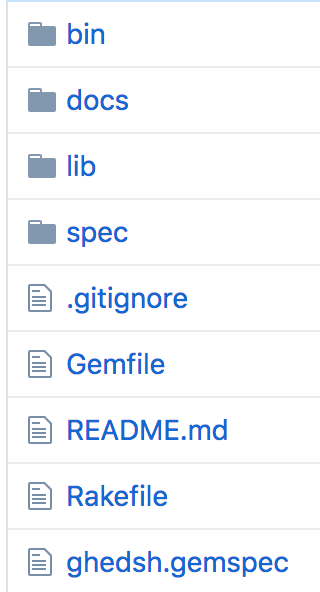
\includegraphics[width=0.20\textwidth]{images/estructura-inicial}
\caption{Estructura del repositorio (primera versión).}
\label{fig:masterv1}
\end{center}
\end{figure}

A continuación, se explicarán los componentes principales del repositorio:
\begin{itemize}
  \item {\it \textbf{bin}}: incluye el ejecutable de la gema, que se cargará en el \verb $PATH  del usuario.
  \item {\it \textbf{lib}}: en este directorio se encuentra el código fuente de la gema.
  \item {\it \textbf{spec}} o {\it \textbf{test}}: aquí se definirán las pruebas, que dependrán del {\it framework} de tests que utilice el desarrollador.
  \item {\it \textbf{Gemfile}}: es un fichero donde se especifican las dependencias del programa.
  \item {\it \textbf{Rakefile}}: se trata de un fichero muy común en las gemas. Su función es, principalmente, la automatización de tareas.
  \item {\it \textbf{gemspec}}: en este último fichero se incluye toda la información acerca de la gema, como, por ejemplo,
  su versión, plataforma soportada, versión de Ruby requerida y nombre y correo electrónico del autor o autores.
\end{itemize}
\bigskip
%----------------------------------------------------------------------
\subsection{Contenido del repositorio}
\label{2.1.2}
El primer paso del análisis consistió en comprender exactamente el flujo del programa. Ésto es necesario dado que, para identificar las partes mejorables del diseño inicial, requiere entenderlo en profundidad.
\bigskip

En la figura \ref{fig:lib}, vemos el contenido de \verb /lib :

\begin{figure}[H]
  \begin{center}
  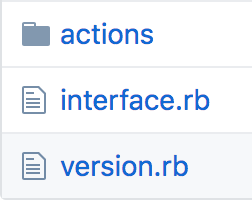
\includegraphics[width=0.25\textwidth]{images/lib}
  \caption{Contenido del directorio lib.}
  \label{fig:lib}
  \end{center}
\end{figure}

Los dos ficheros que ahí se encuentan son: \verb interface.rb  y \verb version.rb  .
\bigskip

En cuanto a \verb interface.rb , implementa la clase {\it Interface}. Ésta clase lleva a cabo el bucle principal característico de los CLI, se trata del bucle {\it Lectura-Evaluación-Impresión}
(en inglés, {\it REPL, Read-Eval-Print-Loop} \cite{B9}), que consiste en:
\begin{itemize}
  \item \textbf{Lectura}: parsea la entrada del usuario y determina si existe esa acción en la estructura de datos interna.
  \item \textbf{Evaluación}: una vez que se acepta la entrada del usuario se ejecutan las acciones con los parámetros especificados, si son necesarios. Es aquí donde se realiza el manejo de errores y excepciones.
  \item \textbf{Impresión}: muestra al usuario el resultado obtenido tras realizar el paso de evaluación.
\end{itemize}

Por otro lado, el fichero \verb version.rb , contiene una constante que indica la versión de la gema {\it ghedsh}. También cabe nombrar que, para asignar un identificador numérico a cada estado del software, se ha utilizado {\it Semantic Versioning} \cite{B10}.
\bigskip

A grandes rasgos, este esquema de control de versiones tiene la estructura {\it MAJOR.MINOR.PATCH}, donde
{\it MAJOR} se incrementa cuando se realizan cambios en la API que no son retrocompatibles. {\it MINOR} se modifica al añadir nuevas funcionalidades que sí son retrocompatibles y, por último, {\it PATCH} varía al corregir {\it bugs} en el software.
Un ejemplo de versión sería:
\begin{itemize}
  \item \verb ghedsh  \verb version  \verb 2.3.6 .
\end{itemize}
\bigskip

En cuanto al directorio \verb /lib/actions , la figura \ref{fig:actions} muestra el contenido del mismo:
\begin{figure}[H]
  \begin{center}
  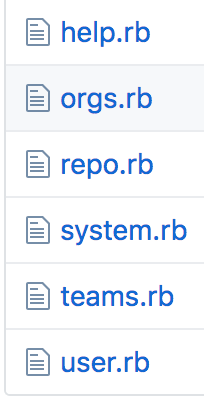
\includegraphics[width=0.17\textwidth]{images/actions}
  \caption{Contenido del directorio actions}
  \label{fig:actions}
  \end{center}
\end{figure}
\bigskip

Los ficheros principales se describirán según la funcionalidad que desempeñan:
\begin{itemize}
  \item \verb orgs.rb : proporciona los métodos necesarios relacionados con las organizaciones para comunicarse con la API de GitHub.
  \item \verb repo.rb : agrupa métodos que llevan a cabo tareas relacionadas con los repositorios, nuevamente, haciendo uso de la API de GitHub.
  \item \verb teams.rb : de manera similar a los anteriores ficheros, especializado en tareas de equipos.
  \item \verb user.rb : agrupa métodos relacionados con el usuario.
  \item \verb system.rb : este fichero se encarga de crear los directorios de configuración de {\it ghedsh}.
\end{itemize}
\bigskip
%--------------------------------------------------------------------------------------
\subsection{Code Smell}
\label{2.1.3}
Una vez analizado el planteamiento inicial, se han detectado una serie de debilidades en el diseño que han dado lugar a diversos {\it code smell} \cite{B11}.
Un {\it code smell} se define como cualquier característica del código fuente que, posiblemente, indica un problema más profundo. No son considerados como {\it bugs}, puesto que no impiden que un programa funcione de manera correcta.
\bigskip

No obstante, estos defectos de diseño pueden afectar al rendimiento del programa, aumentan la probabilidad de errores en el futuro e, incluso, ralentizar el desarrollo del programa y dificultar la extensibilidad del mismo.
\bigskip

Determinar qué es y lo que no es un {\it code smell} para un código fuente específico suele tener un componente de juicio subjetivo, dado que puede variar según el lenguaje de programación utilizado, el desarrollador y la metodología de desarrollo aplicada. Pero, por otro lado, valorar 
los posibles casos de uso, aporta indicaciones para respetar ciertos principios y calidad del software.
\bigskip

En el apartado de refactorización se explicará cómo se ha procedido para solucionarlos. A continuación, se expondrán los {\it code smells} más significativos encontrados en la primera versión de {\it ghedsh}. 
%--------------------------------------------------------------------------------------
  \subsubsection{{\it \textbf{Switch Statements}}}
  Suele ser muy característico de los códigos orientados a objetos. Esencialmente, el problema con las sentencias \verb switch-case  o sentencias \verb if  es la duplicación de código.
  Al utilizarlas con un conjunto de números o cadenas (normalmente, asignadas a constantes) que conforman una lista de valores permitidos para una entidad, existe una dependencia en ellas para decidir la entidad correcta a utilizar en cada momento.
  \bigskip

  Como consecuencia, al añadir nuevos casos, debemos localizar todas estas sentencias en el código y modificarlas.
  Para ilustrarlo con ejemplos, véase las figuras \ref{fig:constantes}, \ref{fig:switch-smell} y \ref{fig:switch-smell2}.
  \bigskip

  \begin{figure}[H]
    \begin{center}
    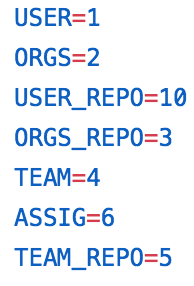
\includegraphics[width=0.18\textwidth]{images/constantes}
    \caption{Constantes numéricas que deciden la entidad a utilizar.}
    \label{fig:constantes}
    \end{center}
  \end{figure}

  \begin{figure}[H]
    \begin{center}
    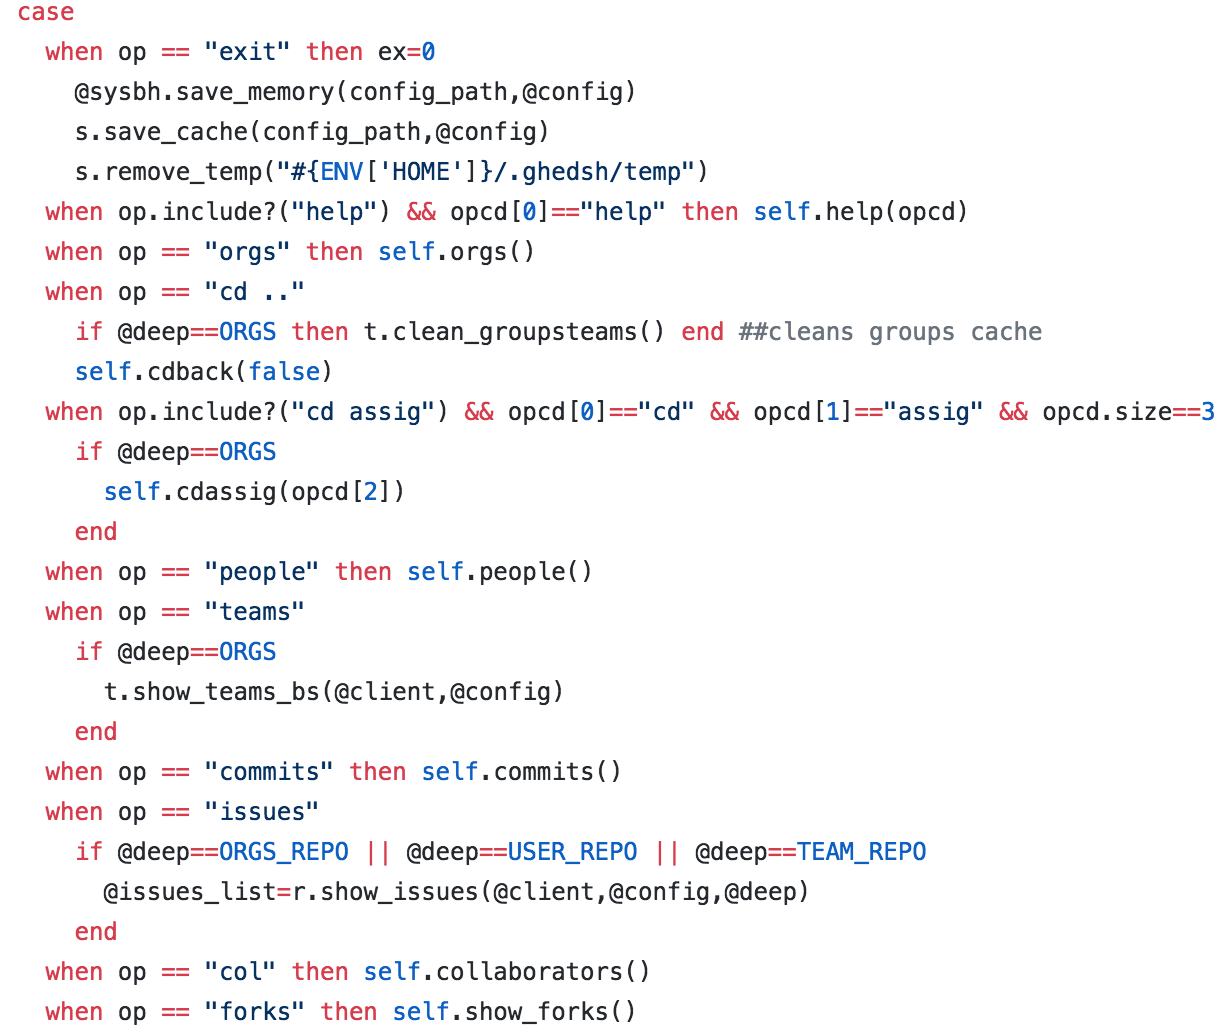
\includegraphics[width=0.89\textwidth]{images/switch-smell}
    \caption{Ejemplo de switch smell, en interface.rb.}
    \label{fig:switch-smell}
    \end{center}
  \end{figure}
  \bigskip

  \begin{figure}[H]
    \begin{center}
    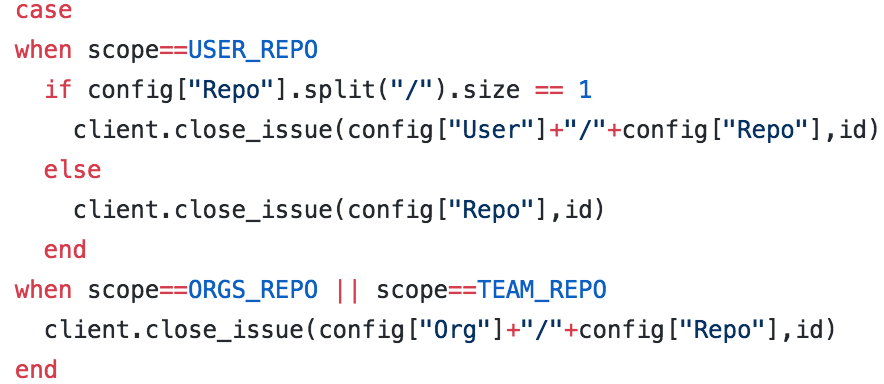
\includegraphics[width=0.70\textwidth]{images/switch-smell2}
    \caption{Otro caso de switch smell, en repo.rb.}
    \label{fig:switch-smell2}
    \end{center}
  \end{figure}
  \bigskip

  Este tipo de {\it smell} es el más repetido a lo largo del código de la primera versión de {\it ghedsh}, por lo que gran parte del proceso de refactorización se ha centrado en este aspecto.
  \bigskip
%-------------------------------------------------------------------------------------
  \subsubsection{{\it \textbf{Long Method}}} 
  Se trata de un {\it smell} que se clasifica a nivel de métodos. Como su nombre indica (método largo), consiste en un método que ha crecido demasiado. 
  \bigskip

  Escribir código suele ser más fácil que interpretarlo. Por ello, muchas veces este {\it smell} pasa desapercibido hasta que el método toma un tamaño considerable y dificulta saber qué es lo que realmente hace. Por esta razón,
  definir métodos más cortos con un nombre significativo, facilita la mantenibilidad del código y su lectura.
  \bigskip
%----------------------------------------------------------------------------
  \subsubsection{{\it \textbf{Large Class}}}
  {\it Large Class} se clasifica dentro de los {\it smells} a nivel de clases. Indica que una clase definida ha crecido excesivamente en tamaño ({\it God Object} \cite{B12}), es decir, realiza demasiadas cosas y que, seguramente, su funcionalidad puede descomponerse
  en clases más pequeñas y fáciles de manejar. Como suele ocurrir en los casos anteriormente nombrados, éste {\it smell} propicia también la duplicación de código.

%---------------------------------------------------------------------------------
\section{Segunda fase: refactorización}
\label{2:sec:2}

En este apartado, se explicará el proceso de refactorización efectuado en el código fuente de {\it ghedsh}. El principal objetivo es el cumplimiento del principio {\it Open/Closed} \cite{B13}, que pertenece a un grupo de cinco principios fundamentales (S.O.L.I.D \cite{B14}) de la programación orientada a objetos y cuya finalidad es
hacer los diseños de software más comprensibles, flexibles y mantenibles.
%-----------------------------------------------------------------------------------
\subsection{Principios de diseño S.O.L.I.D}
\label{2.2.1}
Se desarrollará ahora el significado de este acrónimo:
\begin{itemize}
  \item {\it \textbf{S}ingle responsibility}: establece que una clase debería de tener sólo una responsabilidad, es decir, si fuera necesario modificar dicha clase, debe ser por un único motivo.
  \item {\it \textbf{O}pen/Closed}: una entidad software debería estar abierta para extensión y cerrada para modificación. En el siguiente párrafo se explicará con más detalle este principio.
  \item {\it \textbf{L}iskov substitution}: los objetos de un programa deberían ser sustituíbles por subtipos de ese objeto, sin afectar al correcto funcionamiento de ese programa.
  \item {\it \textbf{I}nterface segregation}: indica que es preferible muchas interfaces cliente específicas, en lugar de una interfaz de propósito general.
  \item {\it \textbf{D}ependency inversion}: sugiere que se debe depender de abstracciones, no de implementaciones. Esto da lugar a la técnica inyección de dependencias.
\end{itemize}
\bigskip

Como se ha indicado anteriormente, se procederá a detallar el principio {\it Open/Closed}, puesto que es bastante necesario desde el punto de vista del desarrollo de {\it ghedsh}. La principal razón es que, si otro desarrollador desea incluir nuevas funcionalidades, no necesitaría cambiar el código original de la gema.
\bigskip

Este principio establece que, las entidades de software, ya sean módulos, funciones, clases, etcétera, deberían estar abiertas para la extensión de su comportamiento, pero cerradas para su modificación. Ésto se consigue, por ejemplo, mediante herencia, reescribiendo los métodos de la clase madre, pudiendo incluso ser abstracta dicha clase.
Otra manera sería por medio de inyección de dependencias, que tienen la misma interfaz pero distinto funcionamiento.

%---------------------------------------------------------------------------------
\subsection{Refactorización: Strategy pattern}
\label{2.2.2}
En esta sección se expondrá el proceso que se ha seguido para eliminar el {\it switch smell}. El proceso ha consistido, fundamentalmente,
en la aplicación del patrón estrategia (en inglés, {\it Strategy pattern} \cite{jspatterns:2012}).
\bigskip

{\it Strategy} es un patrón que permite a un programa seleccionar un algoritmo particular en tiempo de ejecución. El propósito de este patrón es proporcionar una manera clara 
de definir familias de algoritmos, encapsulando cada uno como objeto para poder intercambiarlos fácilmente. El principal beneficio de este modelo es que el objeto cliente puede elegir aquel algoritmo que le conviene y
permutarlo dinámicamente según sus necesidades.
\bigskip

En cuanto a cómo se ha aplicado este patrón, primero ha sido necesario modificar el diseño inicial propuesto en la primera versión de {\it ghedsh}.
De manera que, en el directorio \verb /lib \verb /actions , se han reescrito las clases que allí se encontraban y su propósito también ha cambiado, dado que ya no se agrupan métodos para repositorios, organizaciones, equipos, etcétera, sino que
contendrán las acciones permitidas en cada uno de estos contextos. De este modo, aunque las acciones sean permitidas en varios contextos, cada clase conocerá su propia implementación.
\bigskip

A partir de la segunda versión, en \verb /lib \verb /actions , se encuentran las siguientes clases:
\begin{itemize}
  \item \verb orgs.rb : se define la clase \verb Organization , contiene los métodos de las acciones permitidas para las organizaciones.
  \item \verb system.rb : contiene la clase que se encarga de gestionar los directorios de configuración de {\it ghedsh}, así como guardar la configuración del usuario.
  \item \verb teams.rb : se define la clase \verb Team , que incluye los métodos de las acciones permitidas para los equipos.
  \item \verb user.rb : incluye en la clase \verb User , los métodos correspondientes a las acciones que se permiten en el contexto de usuario.
\end{itemize}
\bigskip

Por otro lado, en \verb /lib/interface.rb  (véase la figura \ref{fig:new-loop}) se tiene un claro ejemplo de patrón estrategia, que se aplica en el bucle Lectura-Evaluación-Impresión (REPL). Esto permite decidir en tiempo de ejecución el comando que el usuario quiere utilizar.
Se parsea lo que ha introducido, de manera que el primer {\it token}, se refiere al nombre del comando deseado. Después, se busca dicho comando en la estructura de datos interna, en este caso, un {\it hash}, que consiste en una colección clave-valor en la que
la clave es el nombre que identifica el comando y el valor es la función que exporta la clase \verb Commands ,   la cual decide si es posible ejecutarlo, verificando si contexto actual responde a la acción solicitada por el usuario.
\begin{figure}[H]
  \begin{center}
  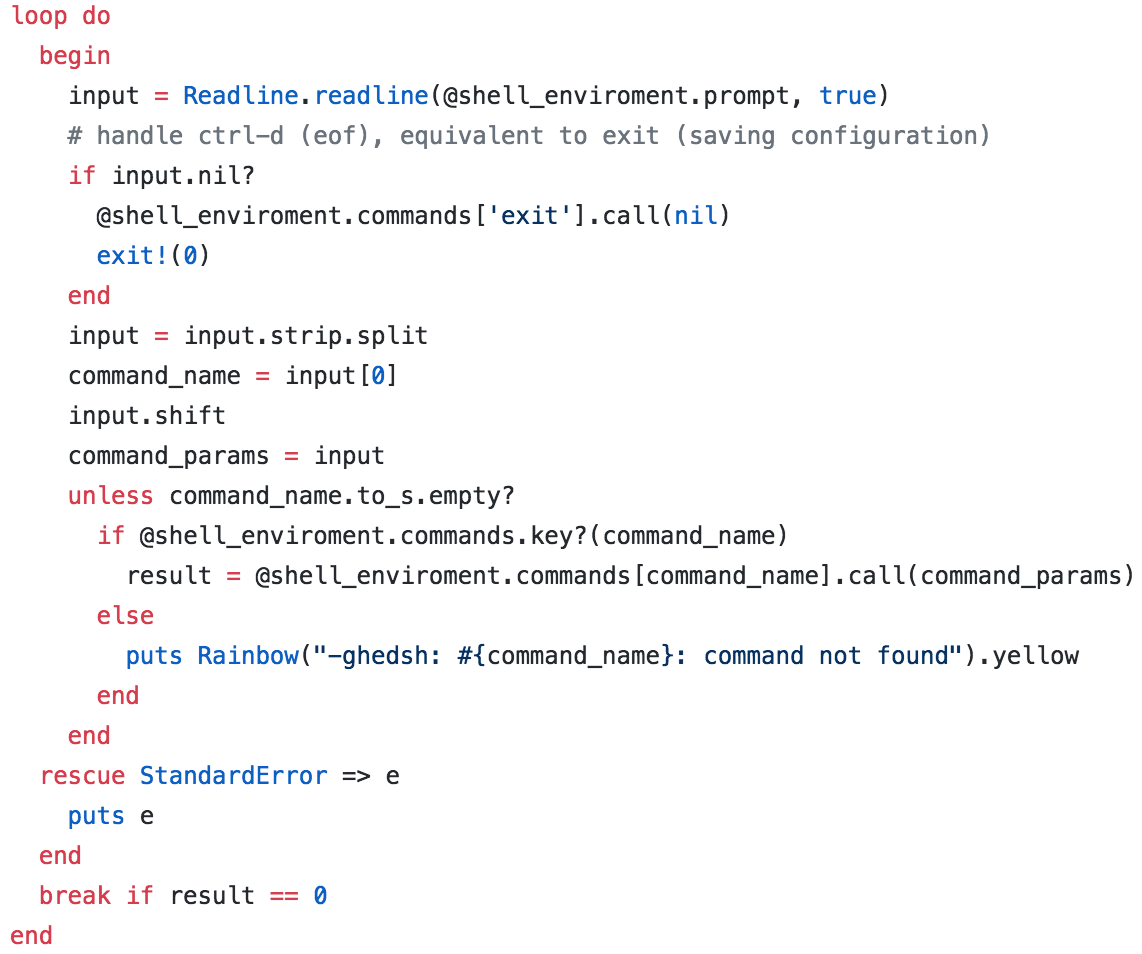
\includegraphics[width=0.80\textwidth]{images/new-loop}
  \caption{Bucle Lectura-Evaluación-Impresión sin sentencia switch/case.}
  \label{fig:new-loop}
  \end{center}
\end{figure}
\bigskip

Cabe destacar que, la figura \ref{fig:switch-smell} anteriormente indicada, representa una porción del código, puesto que ahí se encontraban {\it hard-coded} \cite{B15} todos los comandos.
Sin embargo, en la figura \ref{fig:new-loop} se encuentra todo el código del REPL, tarea en la que se especializa la clase \verb Interface .
\bigskip

Aparte, con este nuevo esquema se logra eliminar las constantes que deciden el tipo de clase a utilizar en cada momento (véase \ref{fig:constantes}), ya que, en esta segunda versión,
existe una variable que almacena el contexto y referencia directamente la clase con la que se realizan las acciones y ya no es necesario hacer la distinción entre, por ejemplo, repositorio de usuario, repositorio de organización y repositorio de equipo. Esto es así porque cada clase gestiona su contexto.
\bigskip

\subsection{Refactorización: Extract Method}
\label{2.2.3}
Como resultado de aplicar el patrón {\it Strategy} y la reescritura de las clases encargadas de las acciones, también se ha solucionado el {\it Long Method smell}. Ésto se ha logrado reduciendo el cuerpo de la función, a través de la extracción de partes del código que realizan tareas similares,
dando lugar a nuevas funciones.
\bigskip

Para ilustrarlo mejor, en la siguiente porción de código vemos un ejemplo de {\it Extract Method} muy simple:
\bigskip 

\begin{minipage}[t]{0.45\linewidth}
  Problema:
  \begin{lstlisting}[language=Ruby]
    def print_owing(amount)
      print_banner

      # print details
      puts "name: #{@name}"
      puts "amount: #{amount}"
    end
  \end{lstlisting}
\end{minipage}
  %
\begin{minipage}[t]{0.5\linewidth}
    Solución (Extract Method):
  \begin{lstlisting}[language=Ruby]
    def print_owing(amount)
      print_banner
      print_details(amount)
    end

    def print_details(amount)
      puts "name: #{@name}"
      puts "amount: #{amount}"
    end
  \end{lstlisting}
\end{minipage}
\bigskip

Si llevamos esto a un programa real, los beneficios son claros:
\begin{itemize}
  \item Código más legible. Hay que destacar que, el nuevo método creado, debe llevar un nombre representativo, es decir, un nombre que describa su propósito.
  \item Menos duplicación de código. Muchas veces, el código contenido en una función puede ser reutilizado en otras partes del programa. Por lo tanto, reemplazamos el código repetido por llamadas al nuevo método.
  \item Mejor detección de errores. Al aislar partes de código, detectar dónde se ha producido un error es más fácil, ya que son menos líneas que revisar.
\end{itemize}




\subsection{Refactorización: Extract Class}
\label{2.2.4}







%%%%%%%%%%%%%%%%%%%%%%%%%%%%%%%%%%%%%%%%%%%%%%%%%%%%%%%%%%%%%%%%%%%%%%%%%%%%%%%
\newpage{\pagestyle{empty}}
\thispagestyle{empty}

\chapter{Resultados obtenidos}
\label{chapter:tres}

%%%%%%%%%%%%%%%%%%%%%%%%%%%%%%%%%%%%%%%%%%%%%%%%%%%%%%%%%%%%%%%%%%%%%%%%%%%%%%%
% Chapter 3: Resultados
%%%%%%%%%%%%%%%%%%%%%%%%%%%%%%%%%%%%%%%%%%%%%%%%%%%%%%%%%%%%%%%%%%%%%%%%%%%%%%%

%++++++++++++++++++++++++++++++++++++++++++++++++++++++++++++++++++++++++++++++
Este capítulo se centrará en explicar las características que incorpora {\it ghedsh} tras la etapa de desarrollo tratada en el capítulo anterior.
\bigskip

Se hará una distinción entre comandos del núcleo y comandos incorporados ({\it built-in commands}). Los comandos del núcleo, son aquellos que no trabajan con los datos de GitHub del usuario pero que, sin embargo, son
esenciales desde el punto de vista la usabilidad y experiencia de usuario con el CLI.
\bigskip

Por otro lado, los comandos incorporados sí trabajan con los datos de GitHub del usuario identificado. Permiten realizar diversas tareas, priorizando la rapidez en la ejecución de las mismas y la facilidad de uso de la herramienta.

%---------------------------------------------------------------------------------
\section{Autenticación con credenciales de GitHub}
\label{3:sec:1}

El contenido de esta sección pretende explicar el proceso de autenticación que debe seguir el usuario al usar {\it ghedsh} por primera vez.
\bigskip

Dicho proceso es necesario, puesto que se trabajan con los datos que dispone el usuario en GitHub. Además, la API REST v3 requiere, para ciertas consultas (en especial, modificaciones como crear repositorios, equipos y administrar la configuración), verificar la identidad del usuario. Si no fuera así, se podrían llevar a cabo comportamientos indeseados.
\bigskip

En {\it ghedsh}, se realiza la autenticación con {\it OAuth access token}\cite{B16}, que consiste, en una definición muy simplificada, en una cadena de caracteres alfanuméricos que actúa como una contraseña. No obstante,
en este caso de uso es mucho más potente y segura. Las principales ventajas son:
\begin{itemize}
	\item Es revocable, es decir, el {\it token} puede dejar de ser válido, eliminando el acceso para ese {\it token} en particular, sin que el usuario tenga que cambiar su contraseña en todos sus accesos.
	\item Sus permisos son configurables, esto es, un {\it token} puede ser válido sólo para ciertos recursos de una API. De esta manera, se conceden permisos de forma más controlada.
\end{itemize}

Para sintetizar este apartado, el usuario que utilice por primera vez {\it ghedsh}, debe verificar su identidad mediante sus credenciales (nombre de usuario y contraseña) de GitHub y se
generará de forma automática un {\it token} de acceso con los permisos necesarios para usar la herramienta.

\begin{figure}[H]
	\begin{center}
	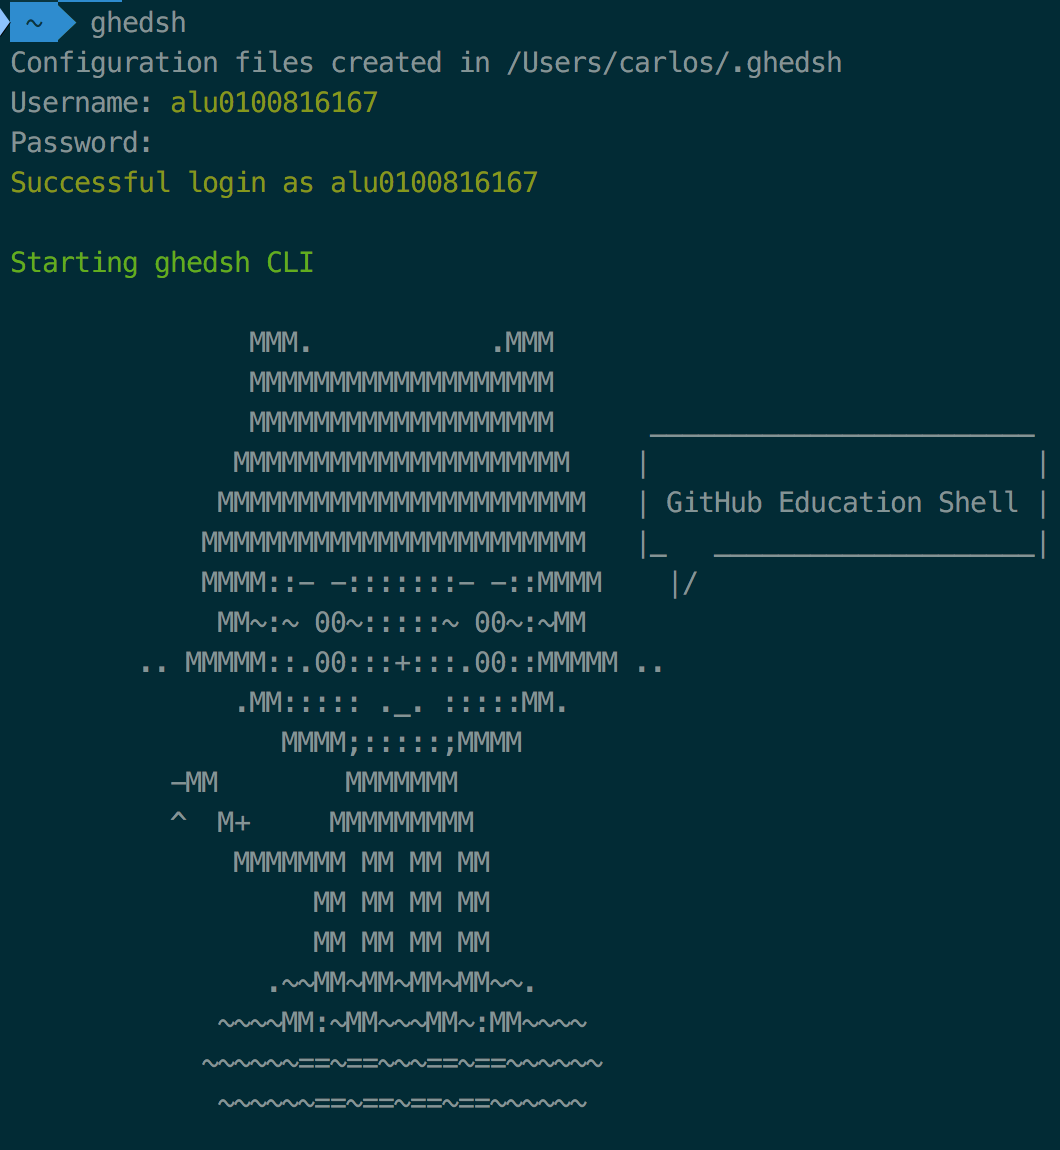
\includegraphics[width=0.45\textwidth]{images/login-example}
	\caption{Ejemplo de autenticación al usar ghedsh por primera vez.}
	\label{fig:masterv1}
	\end{center}
\end{figure}

%------------------------------------------------------------------------------------------------------------
\section{Comandos del núcleo de ghedsh}
\label{3:sec:2}

Como se ha indicado en la introducción de este tercer capítulo, se han separado, por un lado, los comandos del núcleo de {\it ghedsh} y, por otro, los comandos característicos de {\it ghedsh}.
\bigskip

En esta sección, se explicará este primer grupo de comandos, encargado de tareas relacionadas con el sistema operativo y, lo más importante, hacer que la herramienta sea agradable de manejar para el usuario. Además, se revisarán aspectos importantes de su implementación.

\subsection{Change directory: cd}
\label{3.2.1}
Análogamente al comando {\it cd} de la {\it Bash}\cite{B17}, que permite cambiar nuestro directorio actual de trabajo, en {\it ghedsh} también existe este comando. No obstante, aunque la idea es similar, existen diferencias a la hora de usarlo.
\bigskip

En nuestro sistema operativo (tipo Unix)\cite{B18}, cuando realizamos la operación {\it cd}, sólo podemos movernos entre directorios (dependiendo de los permisos). Dado que en {\it ghedsh} no existen directorios como tal, hablaremos de contextos.
Los contextos en esta herramienta hacen referencia a nivel de usuario, nivel de organización, nivel de repositorio, etcétera.
\bigskip

Imaginemos por un momento que nuestro usuario se llama \verb ejemplo , disponemos de un repositorio que se llama \verb ejemplo  y una organización denominada \verb ejemplo . Ésto es totalmente válido, puesto que lo que no permite GitHub es que dos usuarios se llamen igual, que el usuario tenga dos repositorios con el mismo nombre o dos organizaciones bajo el mismo nombre.
Entonces, debemos proporcionar alguna manera de desambiguar a qué contexto nos queremos cambiar.
\bigskip

En {\it ghedsh} se ha optado por el siguiente planteamiento: para realizar la operación de
{\it cd}, es necesario especificar el tipo de contexto (nivel) al que queremos cambiarnos, así, aunque el usuario se encuentre en el caso anteriormente comentado, {\it ghedsh} es capaz de saber a qué contexto debe cambiar.
La sintaxis del comando sería \verb cd  \verb <tipo>  \verb <nombre|Regexp> , donde nombre es la cadena de texto que identifica al tipo, o bien, una expresión regular que mostraría las cadenas que han casado.
\bigskip

Los tipos de contexto (pueden ser ampliables) que actualmente se soportan en {\it ghedsh} son:
\begin{itemize}
	\item \textbf{Nivel de usuario}: estando a nivel de usuario, éste se puede cambiar a cualquiera de sus repositorios o a cualquier organización a la que pertenezca, como vemos a continuación:
		\begin{itemize}
			\item Repositorio del usuario: \verb cd   \verb repo  \verb <nombre|/Regexp/> .
			\item Organización del usuario: \verb cd   \verb org  \verb <nombre|/Regexp/> .
		\end{itemize}
	\item \textbf{Nivel de organización}: estando a nivel de una organización de la que es miembro el usuario autenticado, ({\it ghedsh} sabrá que se refiere al entorno de la organización a la que se ha cambiado) se puede mover a:
		\begin{itemize}
			\item Repositorio de la organización: \verb cd   \verb repo  \verb <nombre|/Regexp/> .
			\item Equipo de la organización: \verb cd   \verb team  \verb <nombre|/Regexp/> .
		\end{itemize}
\end{itemize}

Además, si deseamos volver al contexto anterior, haremos de la misma manera que en sistemas operativos tipo Unix: \verb cd  \verb ..  . Hay que tener en cuenta que, actualmete, no se puede realizar la operación de volver al contexto anterior y cambiar a otro de manera simultánea (como en Unix \verb cd  \verb ../another/dir  ), es necesario hacerlo por separado.


\subsubsection{Detalles de implementación}
Puesto que se trata de uno de los comandos más importantes de {\it ghedsh}, se comentarán los aspectos destacados de la implementación del mismo, incluyendo las dificultades encontradas.
\bigskip

Internamente, el comando {\it cd} contiene una pila (stack\cite{B19}) en la que se almacenan todos los contextos previos. La estructura de un contexto se muestra en el siguiente fragmento de código:

\begin{lstlisting}[language=Ruby]
  config = {
    'User' => client.login.to_s,
  	'user_url' => client.web_endpoint.to_s << client.login.to_s,
    'Org' => nil,
    'org_url' => nil,
    'Repo' => nil,
    'repo_url' => nil,
    'Team' => nil,
    'team_url' => nil
  }
\end{lstlisting}

\begin{itemize}
	\item \verb User : permite saber el nombre del usuario autenticado en {\it ghedsh}.
	\item \verb user_url : contiene la URL ({\it Uniform Resource Locator}\cite{B20}) del perfil del usuairo en GitHub.
	\item \verb Org : indica el nombre de la organización actual, si el usuario no está posicionado sobre alguna, el valor es nulo.
	\item \verb org_url : URL de la organización en GitHub.
	\item \verb Repo : nombre del repositorio actual, en caso de estar dentro de alguno.
	\item \verb repo_url : URL del repositorio en GitHub.
	\item \verb Team : nombre del equipo actual si el usuario está posicionado dentro de alguno.
	\item \verb team_url : URL del equipo en GitHub.
\end{itemize}

En esencia, {\it change directory} irá variando estos parámetros para conocer a qué nivel se encuentra el usuario (\verb User  siempre tendrá un valor asignado porque representa el usuario autenticado).
Por ejemplo, para referirnos a un repositorio de una organización en la que el usuario es miembro, tendríamos:
\begin{lstlisting}[language=Ruby]
	config = {
    'User' => client.login.to_s,
  	'user_url' => client.web_endpoint.to_s << client.login.to_s,
    'Org' => "EXAMPLE-ORG",
    'org_url' => nil,
    'Repo' => "repository-within-example-org",
    'repo_url' => nil,
    'Team' => nil,
    'team_url' => nil
  }
\end{lstlisting}
En el caso de un repositorio de usuario, \verb User  tendría valor asignado y \verb Repo  también tendría valor asignado. A diferencia con el caso anterior, \verb Org  sería nulo ya que nos referimos a un repositorio a nivel de usuario.
\bigskip

Una de las dificultades en la implementación de este comando, fue que, antes de reasignar la estructura de datos que respresenta los contextos, era necesario almacenar el contexto actual para poder volver a éste más tarde.
\bigskip

Ruby proporciona dos métodos para copiar/clonar objetos: \verb dup \cite{B21} y \verb clone \cite{B22}. No obstante, realizan una copia superficial del objeto, es decir, crearán un nuevo identificador de objeto pero
el contenido del mismo referenciará al de la entidad original.
\bigskip

Para solucionarlo, se utilizó el módulo {\it Marshal}\cite{B23} de Ruby, que sí realiza una copia profunda del objeto.

\subsection{Bash (comando ghedsh)}
\label{3.2.1}

Permite interpretar un comando en la terminal del sistema operativo, sin salir de {\it ghedsh}.
\bigskip

\textbf{Sintaxis:} \verb bash  \verb <comando_terminal>  .
En la figura \ref{fig:bash-example}, se muestra un ejemplo de uso.
\begin{figure}[H]
	\begin{center}
	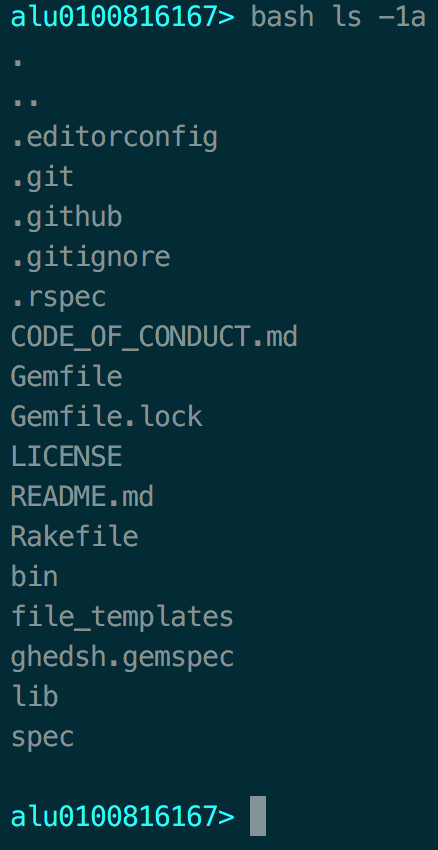
\includegraphics[width=0.30\textwidth]{images/bash-example}
	\caption{Ejemplo de uso del comando bash.}
	\label{fig:bash-example}
	\end{center}
\end{figure}

%------------------------------------------------------------------------------------------------------------
\section{Comandos incorporados en ghedsh}
\label{3:sec:3}   
    

%------------------------------------------------------------------------------------------------------------
\section{Comandos que facilitan el proceso de evaluación}
\label{3:sec:4}




%%%%%%%%%%%%%%%%%%%%%%%%%%%%%%%%%%%%%%%%%%%%%%%%%%%%%%%%%%%%%%%%%%%%%%%%%%%%%%%
\newpage{\pagestyle{empty}}
\thispagestyle{empty}

\chapter{Conclusiones y líneas futuras}
\label{chapter:Conclusiones}

%%%%%%%%%%%%%%%%%%%%%%%%%%%%%%%%%%%%%%%%%%%%%%%%%%%%%%%%%%%%%%%%%%%%%%%%%%%%%
% Chapter 4: Conclusiones y Trabajos Futuros 
%%%%%%%%%%%%%%%%%%%%%%%%%%%%%%%%%%%%%%%%%%%%%%%%%%%%%%%%%%%%%%%%%%%%%%%%%%%%%%%

%++++++++++++++++++++++++++++++++++++++++++++++++++++++++++++++++++++++++++++++

Desde hace unos años hasta ahora, ha tenido lugar un enorme crecimiento de las herramientas de control de versiones. Se han convertido en una herramienta imprescindible en la metodologías de desarrollo del software y las instituciones de enseñanza saben que incorporarlas a sus sistemas educativos es clave para ofrecer un servicio puntero y de calidad.
\bigskip

Ésto es lo que se pretende con la herramienta obtenida tras la realización de este Trabajo de Fin de Máster: que sea posible su implantación dentro del marco académico de la Universidad de La Laguna, partiendo de la premisa de que, actualmente, el desarrollo de un proyecto software sin tener detrás un sistema de control de versiones, no es viable.
\bigskip

La automatización de las tareas de clonado y ejecución de pruebas facilitaría al profesor, en primera instancia, la corrección de las prácticas y proyectos de los alumnos. El ahorro de tiempo de ejecutar estas tareas manualmente es considerable, teniendo en cuenta el número de prácticas que realiza cada alumno por asignatura. Esta enorme carga de trabajo del profesor puede ser aprovechada en otros ámbitos docentes.
\bigskip

Por otra parte, esta herramienta sienta las bases a posibles desarrollos futuros, ampliando las funcionalidades de la misma. Se ha desarrollado pensando en su posible escalabilidad y ya que cuenta con toda la estructura base creada (autentificación de usuarios, clonado, ejecución y reporte de resultados), se pueden añadir funcionalidades sin demasiado esfuerzo.
\newpage

Para concluir, podemos afirmar que los objetivos marcados al comienzo de este Trabajo de Fin de Máster han sido cumplidos y las principales líneas de desarrollo a continuar podrían ser las enumeradas a
continuación:  

\begin{itemize}
	\item Dotar de más funcionalidad de GitHub a la herramienta:
	\begin{itemize}
		\item Subir cambios a los repositorios (git push).
		\item Crear issues.
		\item Gestionar Pull Requests.
		\item Buscar repositorios.
		\item Gestión de permisos de usuarios a repositorios y organizaciones.
		\item Gestionar Classrooms.
	\end{itemize}
	\item Enriquecer el formato de la documentación generada.
	\item Realizar despliegues locales de aplicaciones web (como procesos hijos de la herramienta).
\end{itemize}



%%%%%%%%%%%%%%%%%%%%%%%%%%%%%%%%%%%%%%%%%%%%%%%%%%%%%%%%%%%%%%%%%%%%%%%%%%%%%%%
\newpage{\pagestyle{empty}}
\thispagestyle{empty}

\chapter{Summary and Conclusions}
\label{chapter:ingles}

%%%%%%%%%%%%%%%%%%%%%%%%%%%%%%%%%%%%%%%%%%%%%%%%%%%%%%%%%%%%%%%%%%%%%%%%%%%%%
% Chapter 5: Summary and Conlusions
%%%%%%%%%%%%%%%%%%%%%%%%%%%%%%%%%%%%%%%%%%%%%%%%%%%%%%%%%%%%%%%%%%%%%%%%%%%%%%%

%++++++++++++++++++++++++++++++++++++++++++++++++++++++++++++++++++++++++++++++

This chapter is compulsory.
The memory should include an extended summary and conclusions in english. 

%---------------------------------------------------------------------------------
\section{First Section}
\label{5:sec:1}



%%%%%%%%%%%%%%%%%%%%%%%%%%%%%%%%%%%%%%%%%%%%%%%%%%%%%%%%%%%%%%%%%%%%%%%%%%%%%%%
\newpage{\pagestyle{empty}}
\thispagestyle{empty}

\chapter{Presupuesto}
\label{chapter:presupuesto}

%%%%%%%%%%%%%%%%%%%%%%%%%%%%%%%%%%%%%%%%%%%%%%%%%%%%%%%%%%%%%%%%%%%%%%%%%%%%%
% Chapter 6: Summary and Conlusions
%%%%%%%%%%%%%%%%%%%%%%%%%%%%%%%%%%%%%%%%%%%%%%%%%%%%%%%%%%%%%%%%%%%%%%%%%%%%%%%

%++++++++++++++++++++++++++++++++++++++++++++++++++++++++++++++++++++++++++++++

CodeLab was born as a tool that aims to extend the functionality
of other tools such as Github Classroom, adding specific functions
for the teachers to support the management of courses and 
the correction of programming labs.

The platform has been designed with ease of use in mind for those
who are not familiar with GitHub. On the other hand, emphasis has
been placed on fulfilling the Free Software standards as much as
possible,
facilitating collaborative development and the inclusion of new features by other programmers.

We believe that the facilities provided by  CodeLab are
useful for lecturers who have large groups of students
or who are not familiar with the Github environment.

Version control offers many advantages to developers.
Currently, most development companies use the git version control system, 
and consequently it is essential that students learn to handle git correctly and
learn teamwork techniques as well as all the tools that Github
provides such as issues or projects.

In the future, I would like to continue developing CodeLab, improving
it and adding new functionalities. One of the first improvements
that is proposed is the use of a front-end library such as Vue or
React to improve the visual quality of the web platform. A new
functionality that I would like to add is the possibility of more
than one teacher per classroom.


%%%%%%%%%%%%%%%%%%%%%%%%%%%%%%%%%%%%%%%%%%%%%%%%%%%%%%%%%%%%%%%%%%%%%%%%%%%%%%%
\newpage{\pagestyle{empty}}
\thispagestyle{empty}
\begin{appendix}

\chapter{Glosario}
\label{appendix:1}
{\bfseries {\Huge A}}\label{Apendice1:A}
\bigskip
\bigskip

\begin{description}
  \item[\underline{AJAX}\label{apend1:ajax}]: acr\'onimo de \textit{Asynchronous JavaScript And XML} (JavaScript as\'{\i}ncrono y XML). Es una t\'ecnica de desarrollo web para crear aplicaciones 
  interactivas o RIA (\textit{Rich Internet Applications}). Estas aplicaciones se ejecutan en el cliente, es decir, en el navegador de los usuarios mientras se 
  mantiene la comunicaci\'on as\'{\i}ncrona con el servidor en segundo plano. De esta forma es posible realizar cambios sobre las p\'aginas sin necesidad de 
  recargarlas, mejorando la interactividad, velocidad y usabilidad en las aplicaciones.
  \bigskip
\end{description}

\begin{description}
  \item[\underline{API}\label{apend1:api}]: (\textit{Application Programming Interface} o Interfaz de Programaci\'on de Aplicaciones). Conjunto de funciones y procedimientos o m\'etodos que 
  ofrece cierta librer\'{\i}a para ser utilizados por otro software como una capa de abstracci\'on. 
  \bigskip
\end{description}

\begin{description}
  \item[\underline{Asíncrono}\label{apend1:asincrono}]: 
  \bigskip
\end{description}

\begin{description}
  \item[\underline{Asignación}\label{apend1:asignacion}]: 
  \bigskip
\end{description}

\begin{description}
  \item[\underline{Async/Await}\label{apend1:async-await}]: 
  \bigskip
\end{description}


\bigskip
{\bfseries {\Huge C}}\label{Apendice1:C}
\bigskip
\bigskip

\begin{description}
   \item[\underline{CVS}\label{apend1:cvs}]: (\textit{Control Versioning System} o Sistema de Control de Versiones). Aplicaci\'on inform\'atica que implementa un sistema de control de 
  versiones: mantiene el registro de todo el trabajo y los cambios en los ficheros (c\'odigo fuente principalmente) que forman un proyecto y permite que distintos desarrolladores 
  (potencialmente situados a gran distancia) colaboren.
  \bigskip
\end{description}


{\bfseries {\Huge G}}\label{Apendice1:G}
\bigskip
\bigskip

\begin{description}
  \item[\underline{GitBook}\label{apend1:gitbook}]: 
  \bigskip
\end{description}

\begin{description}
  \item[\underline{GitHub}\label{apend1:github}]: forja para alojar proyectos utilizando el Sistema de Control de Versiones {\bfseries Git}. Para m\'as informaci\'on, visitar {\small 
  \url{https://github.com}}.
  \bigskip
\end{description}

\begin{description}
  \item[\underline{GitHub Classroom}\label{apend1:github-classroom}]:
  \bigskip
\end{description}

\bigskip
{\bfseries {\Huge H}}\label{Apendice1:H}
\bigskip
\bigskip

\begin{description}
  \item[\underline{HTML5}\label{apend1:html}]: (\textit{HyperText Markup Language}). Lenguaje de marcado para la elaboraci\'on de p\'aginas web. Es un est\'andar que sirve de referencia para la 
  elaboraci\'on de p\'aginas web definiendo una estructura b\'asica y un c\'odigo para la definici\'on del contenido de la misma.
  \bigskip
\end{description}

\bigskip
\newpage

{\bfseries {\Huge J}}\label{Apendice1:J}
\bigskip
\bigskip

\begin{description}
  \item[\underline{JavaScript}\label{apend1:js}]: lenguaje de programaci\'on interpretado. Se define como orientado a objetos, basado en prototipos, imperativo, d\'ebilmente tipado y 
  din\'amico. Se utiliza principalmente en su forma del lado del cliente (\textit{client-side}), implementado como parte de un navegador web permitiendo mejoras en la interfaz de usuario y p\'aginas 
web din\'amicas.
  \bigskip
\end{description}

\bigskip
{\bfseries {\Huge M}}\label{Apendice1:M}
\bigskip
\bigskip

\begin{description}
  \item[\underline{Metodologias \'agiles}\label{apend1:ma}]: conjunto de m\'etodos de ingenier\'{\i}a del software basados en el desarrollo iterativo e incremental, donde los requisitos y 
  soluciones evolucionan mediante la colaboraci\'on de grupos auto organizados y multidisciplinarios. Se caracterizan adem\'as por la minimizaci\'on de riesgos desarrollando software en
  iteraciones cortas de tiempo.
  \bigskip
\end{description}

\bigskip
{\bfseries {\Huge N}}\label{Apendice1:N}
\bigskip
\bigskip

\begin{description}
  \item[\underline{Node.js}\label{apend1:node}]:
  \bigskip
\end{description}

\begin{description}
  \item[\underline{NPM}\label{apend1:npm}]:
  \bigskip
\end{description}

\bigskip
{\bfseries {\Huge O}}\label{Apendice1:O}
\bigskip
\bigskip

\begin{description}
  \item[\underline{Organización}\label{apend1:organizacion}]:
  \bigskip
\end{description}

\bigskip
{\bfseries {\Huge P}}\label{Apendice1:P}
\bigskip
\bigskip

\begin{description}
  \item[\underline{Promesa}\label{apend1:promesa}]:
  \bigskip
\end{description}

\bigskip
{\bfseries {\Huge R}}\label{Apendice1:R}
\bigskip
\bigskip

\begin{description}
  \item[\underline{Repositorio}\label{apend1:repositorio}]:
  \bigskip
\end{description}

{\bfseries {\Huge S}}\label{Apendice1:S}
\bigskip
\bigskip

\begin{description}
  \item[\underline{Student Developer Pack}\label{apend1:sdp}]: 
  \bigskip
\end{description}

\begin{description}
  \item[\underline{Síncrono}\label{apend1:sincrono}]: 
  \bigskip
\end{description}

{\bfseries {\Huge T}}\label{Apendice1:T}
\bigskip
\bigskip

\begin{description}
  \item[\underline{Travis-CI}\label{apend1:travis}]:
  \bigskip
\end{description}

\begin{description}
  \item[\underline{TDD}\label{apend1:tdd}]: (\textit{Test-Driven Development} o Desarrollo Dirigido por Pruebas). Pr\'actica de programaci\'on que involucra otras dos pr\'acticas: escribir las 
  pruebas primero (\textit{Test First Development}) y Refactorizaci\'on de c\'odigo (\textit{Refactoring}).
  \bigskip
\end{description}

\begin{description}
  \item[\underline{Token}\label{apend1:token}]:
  \bigskip
\end{description}

\bigskip
{\bfseries {\Huge W}}\label{Apendice1:W}
\bigskip
\bigskip

\begin{description}
  \item[\underline{Web sem\'antica}\label{apend1:web}]: idea de a\~{n}adir metadatos sem\'anticos y ontol\'ogicos a la World Wide Web. Esas informaciones adicionales, que describen el contenido, 
  el significado y la relaci\'on de los datos, se deben proporcionar de manera formal, para que sea posible evaluarlas autom\'aticamente por m\'aquinas de procesamiento. El objetivo es mejorar 
  Internet ampliando la interoperabilidad entre los sistemas inform\'aticos usando {\bfseries agentes inteligentes}, es decir, programas en las computadoras que buscan informaci\'on sin necesidad de 
  interacci\'on humana.
  \bigskip
\end{description}

\begin{description}
  \item[\underline{World Wide Web}\label{apend1:www}]: (WWW). Sistema de distribuci\'on de documentos de hipertexto o hipermedios interconectados y accesibles v\'{\i}a Internet. Con un navegador 
  web, un usuario visualiza sitios web compuestos de p\'aginas web que pueden contener texto, im\'agenes, v\'{\i}deos u otros contenidos multimedia, y navega a trav\'es de esas p\'aginas usando 
hiperenlaces.
  \bigskip
\end{description}

\chapter{Guía del desarrollador}
\label{appendix:2}
Esta guía está especialmente dirigida a los desarrolladores que deseen ampliar o mejorar el diseño de {\it ghedsh}, así como incorporar nuevas funcionalidades.
\bigskip

Antes de empezar con el contenido, cabe comentar que se anima a que cada desarrollador incorpore nuevas ideas propias. Por lo tanto, cualquier
aspecto del diseño que sea mejorable, no dude en implementar su idea.

%---------------------------------------------------------------------------------
\section{Instalación}
\label{Apendice2:instalacion}

\subsection{Requisitos}
\label{subsec:b.1.1}

Node.js \textgreater = 8

\subsection{Dependencias}
\label{subsec:b.1.2}

Gitbook
Calibre

\subsection{Instalación}
\label{subsec:b.1.3}

Para instalar el paquete, basta con ejecutar el siguiente comando:
\begin{verbatim}
[~]$ npm install ghshell -g
\end{verbatim}

%---------------------------------------------------------------------------------
%---------------------------------------------------------------------------------

\section{Ejecución}
\label{Apendice2:ejecucion}

\begin{lstlisting}[language=JavaScript]
var foo = function(){
console.log('foo');
}
foo();
\end{lstlisting}
\bigskip

%---------------------------------------------------------------------------------
\subsection{Otras consideraciones}
\label{subsec:Apendice2.1}

Para que

\end{appendix}

%%%%%%%%%%%%%%%%%%%%%%%%%%%%%%%%%%%%%%%%%%%%%%%%%%%%%%%%%%%%%%%%%%%%%%%%%%%%%%%
\addcontentsline{toc}{chapter}{Bibliografía}
\bibliographystyle{plain}%{ieeetr}

\bibliography{TFG}
\nocite{*}

%%%%%%%%%%%%%%%%%%%%%%%%%%%%%%%%%%%%%%%%%%%%%%%%%%%%%%%%%%%%%%%%%%%%%%%%%%%%%%%

\end{document}
